\subsection{Grace Period Detection} \label{sec:grace_period}
Once each CPU has passed through a quiescent state, a grace period for RCU
has completed. 
As discussed in Section \ref{sec:data_structure}, Tree-RCU uses a hierarchy 
of \co{rcu_node} structures to manage quiescent state and grace period
information.
Quiescent-state information is passed up the 
tree from the leaf per-CPU \co{rcu_data} structures.
Grace-period information is passed down from the root.
%
%The dyntick-idle mechanisms used for idle CPUs and \co{nohz_full} userspace
%execution are out of scope for this research, as are RCU CPU stall warnings. The focus is instead 
We focus on grace-period detection for busy CPUs, as illustrated
in Figure~\ref{fig:grace_period_state_diagram}.

\begin{figure}[tb]
\centering
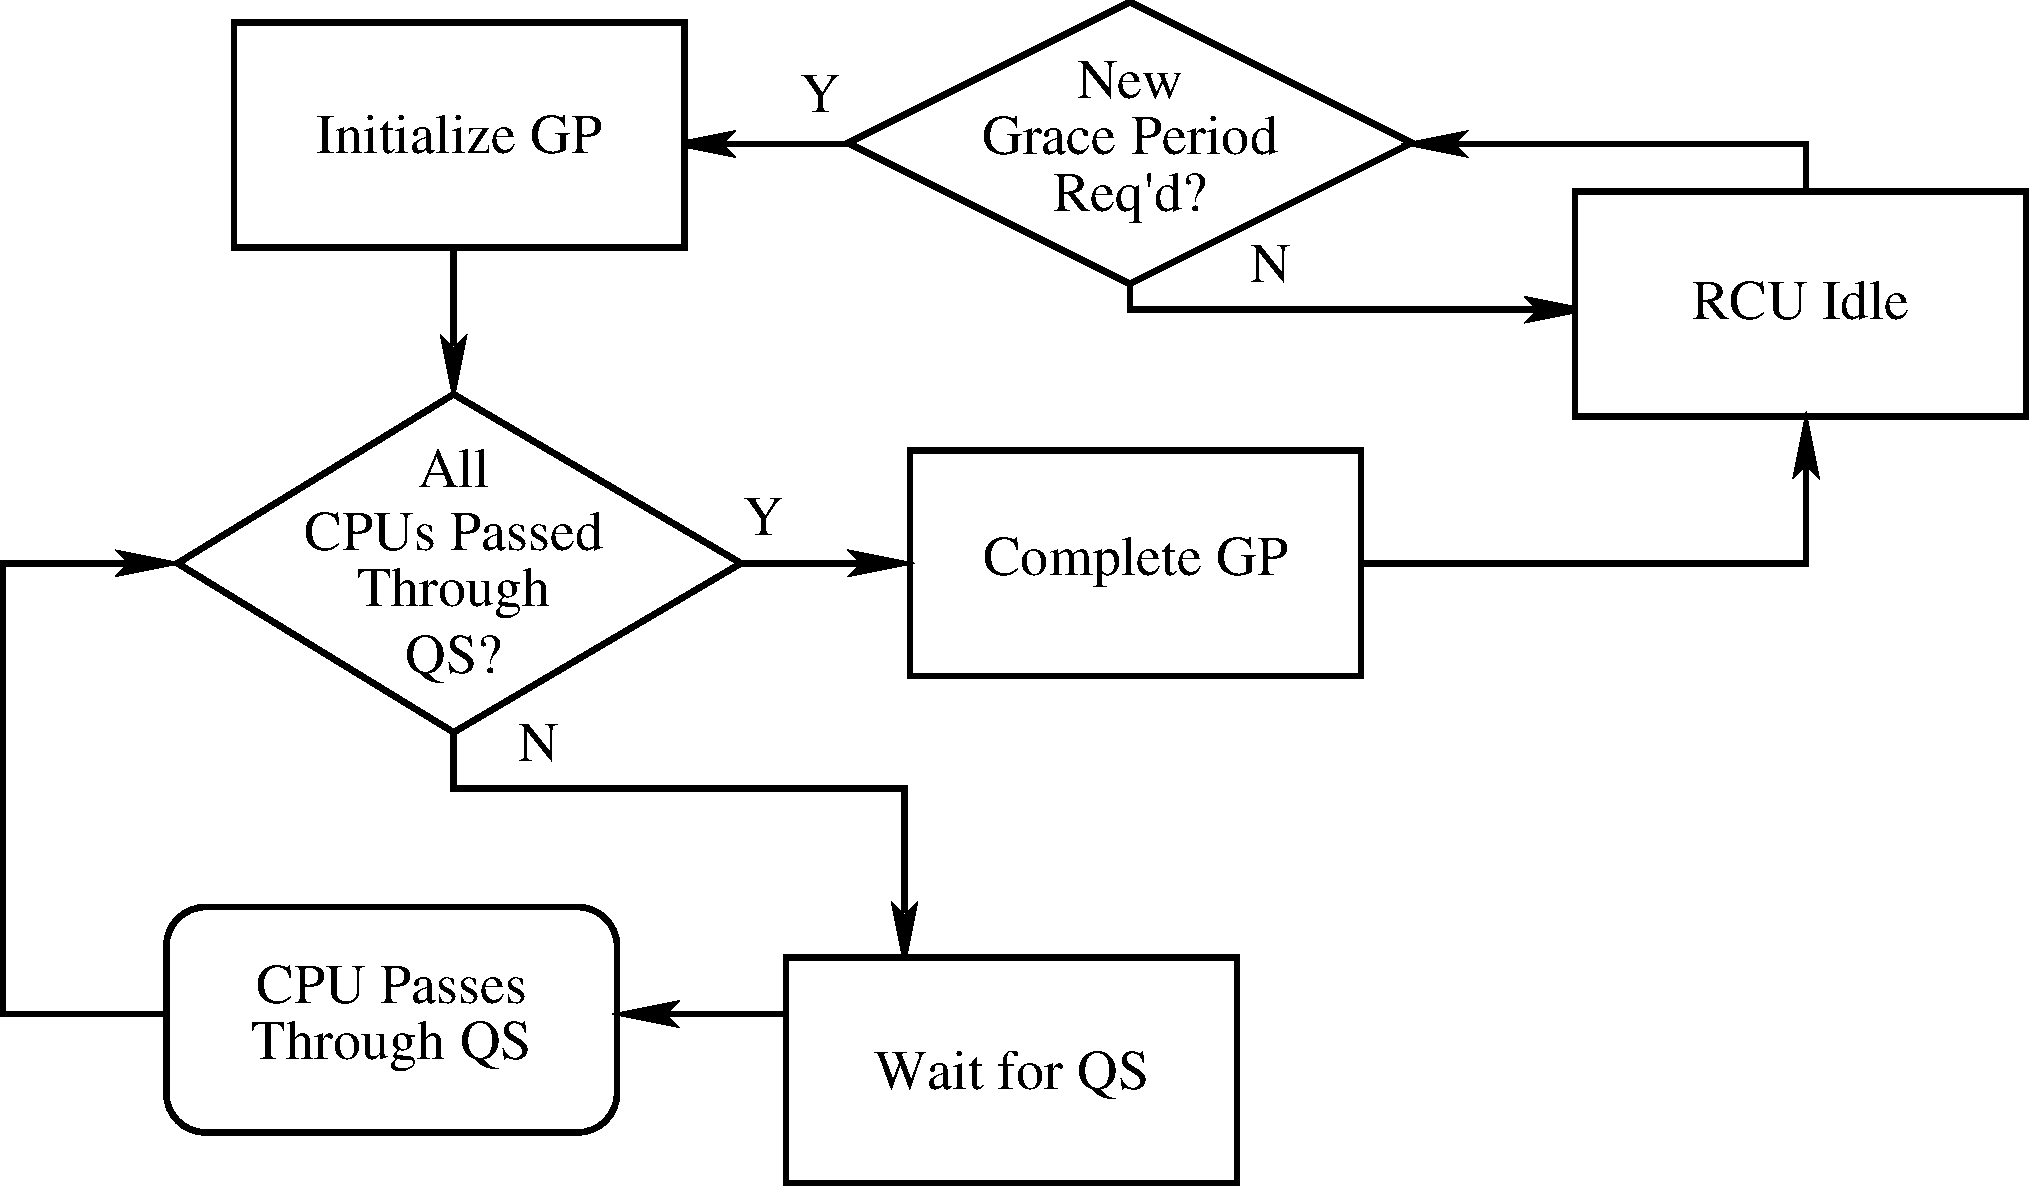
\includegraphics[scale=0.25]{grace_period_state_diagram.pdf}
\caption{Grace-Period Detection State Diagram}
\label{fig:grace_period_state_diagram}
\end{figure}

\subsubsection{Softirq Handler for RCU} \label{sec:rcu_softirq}
RCU's busy-CPU grace period detection relies on the
\co{RCU_SOFTIRQ} handler function \co{rcu_process_callbacks()},
which is scheduled from the scheduling-clock interrupt.
This function first calls
\co{rcu_check_quiescent_state()} to report recent quiescent states
on the current CPU.
Then \co{rcu_process_callbacks()} starts a new grace period if needed,
and finally calls \co{invoke_rcu_callbacks()} to invoke any callbacks
whose grace period has already elapsed.

Function \co{rcu_check_quiescent_state()} first invokes \co{note_gp_changes()} 
to update the CPU-local \co{rcu_data} structure to record the end of 
previous grace periods and the beginning of new grace periods.
%, which are detected via differences in the \co{->completed} and
%\co{->gpnum} fields, respectively.
Any new values for these fields are copied from the leaf \co{rcu_node}
structure to the \co{rcu_data} structure.
If an old grace period has ended, \co{rcu_advance_cbs()} is invoked to
advance all callbacks, otherwise, \co{rcu_accelerate_cbs()} is invoked
to assign a grace period to any recently arrived callbacks.
If a new grace period has started, \co{->passed_quiesce} is set to zero,
and if in addition RCU is waiting for a quiescent state from this CPU,
\co{->qs_pending} is set to one, so that a new quiescent state will
be detected for the new grace period.
%
% Lihao: this is one of the two places where qs_pending gets updated in Tree RCU
% \comment{(Lihao: does it mean even this softirq is invoked because of a quiescent state of this CPU
%   (\co{rdp->passed_quiesce} is set to 1 in \co{rcu_check_callbacks} so \co{rcu_pending} 
%   return 1), if for some reason gpnum in \co{rcu_data} of this CPU is one lag behind its parent 
%   counterpart, this CPU needs to wait for its next quiescent to commit? 
%   \url{http://lxr.free-electrons.com/source/kernel/rcu/tree.c#L1747}
% )}
% Paul: Yes.  I did look into immediately detecting quiescent states for
% RCU-preempt, but it didn't seem worth the coding contortions required.

Next,
\co{rcu_check_quiescent_state()} checks whether \co{->qs_pending} indicates
that RCU needs a quiescent state from this CPU.
If so, it checks whether \co{->passed_quiesce} indicates that this
CPU has in fact passed through a quiescent state.
If so, it invokes \co{rcu_report_qs_rdp()} to report that quiescent
state up the %\co{rcu_data} and \co{rcu_node} 
combining tree.

The \co{rcu_report_qs_rdp()} function first verifies that the CPU has
in fact detected a legitimate quiescent state for the current grace period,
and under the protection of the leaf \co{rcu_node} structure's \co{->lock}.
If not, it resets quiescent-state detection and returns, thus ignoring
any redundant quiescent states belonging to some earlier grace period.
Otherwise, if the \co{->qsmask} field indicates that RCU needs to report a 
quiescent state from this CPU, \co{rcu_accelerate_cbs()} is invoked to assign 
a grace-period number to any new callbacks, and then \co{rcu_report_qs_rnp()} 
is invoked to report the quiescent state to the \co{rcu_node} combining tree.

% \comment{(Lihao: did we just check this in \co{rcu_check_quiescent_state()}? 
%   \url{http://lxr.free-electrons.com/source/kernel/rcu/tree.c#L2394}
% )}
% \comment{(Lihao: but did we just update \co{rdp->gpnum = rnp->gpnum} in \co{note_gp_changes()}...?
%   are they just double-checks or something may happen in between which I miss?
% )}
% Paul:  The code could probably be simplified.  The first step is to
% add assertions to verify the suspicions, and if the assertions don't
% trigger over a period of a year or so, simplify the code.  Sometimes
% the assertions have triggered, hence the caution.  ;-)
%
% \comment{(Lihao: what are \co{rcu_qs_ctr} and \co{rcu_qs_ctr_snap} used for? 
%  \url{http://lxr.free-electrons.com/source/kernel/rcu/tree.c#L2341}
% )}
% Paul: These are used by cond_resched_rcu_qs(), which records a quiescent
% state for all flavors of RCU.
%
%
% \comment{(Lihao: can we use \co{rdp->qs_pending} in the following line of code since 
%  it's also get updated in \co{note_gp_changes()}, right? 
%  \url{http://lxr.free-electrons.com/source/kernel/rcu/tree.c#L2357}
%)}
%
% \comment{(Lihao: comments in \url{http://lxr.free-electrons.com/source/kernel/rcu/tree.c#L2272}
%   say if this CPU is the last one to pass through a quiescent state in the current grace period, 
%   \co{rcu_report_qs_rsp()} is invoked to do the clean up and let \co{rcu_start_gp()} 
%   start a new grace period if one is needed.~But where is \co{rcu_start_gp()} called in 
%   \co{rcu_report_qs_rsp()}?
% )}
% Paul: This is done indirectly by waking up the RCU grace-period kthread.

The \co{rcu_report_qs_rnp()} function traverses up the \co{rcu_node} tree,
at each level holding the \co{rcu_node} structure's \co{->lock}.
At any level, if the child structure's \co{->qsmask} bit is already clear,
or if the \co{->gpnum} changes, traversal stops.
Otherwise, the child structure's bit is cleared from \co{->qsmask},
after which, if \co{->qsmask} is non-zero, %or if any tasks are queued on the
%\co{->blkd_tasks} list (which applies only to RCU-preempt), 
traversal stops. Otherwise, traversal proceeds on to the parent \co{rcu_node} structure.
%If there is no parent (that is, the previous \co{rcu_node} structure was the root), 
%the current grace period has completed. In that case, traversal stops and 
Once the root is reached, traversal stops and \co{rcu_report_qs_rsp()} is
invoked to awaken the grace-period kthread (kernel thread).
The grace-period kthread will then clean up after the now-ended grace
period, and, if needed, start a new one.

\subsubsection{Grace-Period Kernel Thread} \label{sec:rcu_gp_kthread}
The RCU grace-period kthread invokes \co{rcu_gp_kthread()}, which
contains an infinite loop that initializes, waits for, and cleans up after
each grace period. 

% rcu_gp_init()
When no grace period is required, the grace-period kthread
sets its \co{rcu_state} structure's \co{->flags} field to
\co{RCU_GP_WAIT_GPS}, and then
waits within an inner infinite loop for that structure's
\co{->gp_state} field to be set.
Once set, \co{rcu_gp_kthread()} invokes \co{rcu_gp_init()} to initialize
a new grace period, which
rechecks the \co{->gp_state} field under
the root \co{rcu_node} structure's \co{->lock}.
If the field is no longer set, \co{rcu_gp_init()} returns zero.
Otherwise, it
increments \co{rsp->gpnum} by 1 to record a new grace period number.
%
Finally, it performs a breadth-first traversal of the \co{rcu_node}
structures in the combining tree.
For each \co{rcu_node} structure \co{rnp},
% drop preemptible RCU contents
%we invoke \co{rcu_preempt_check_blocked_tasks()}, which responds to
%a non-empty list of blocked tasks by setting \co{rnp->gp_tasks} to
%\co{rnp->blkd_tasks.next}, so that those tasks block the new grace period.
%
we set the \co{rnp->qsmask} to indicate which children
must report quiescent states for the new grace period (Section 
\ref{sec:rcu_node}), and set \co{rnp->gpnum} and \co{rnp->completed}
to their \co{rcu_state} counterparts. 
%
If the \co{rcu_node} structure \co{rnp} is the parent of the current CPU's \co{rcu_data}, 
we invoke \co{__note_gp_changes()} to set up the CPU-local \co{rcu_data} state. 
Other CPUs will invoke \co{__note_gp_changes()} after their next
scheduling-clock interrupt. %(Section~\ref{sec:timer_interrupt}).
 
%Note that other CPUs will access only the leaves of the hierarchy, thus seeing that 
%no grace period is in progress, at least until the corresponding leaf node has been 
%initialized. In addition, we have included CPU-hotplug operations since v4.1.

% Lihao: include this in PhD thesis; also look for 'preemptible RCU contents'
% rcu_gp_fqs()
%During a grace period, the grace-period kthread periodically
%calls \co{force_qs_rnp()} to detect idle and offline CPUs. 
%For each such CPU, \co{force_qs_rnp()} invokes \co{rcu_report_qs_rnp()}
%to report a quiescent state on its behalf, thus avoiding the degraded
%energy efficiency that would be incurred should RCU awaken idle CPUs.
%CPUs that fail to report quiescent states will be sent an
%inter-processor interrupt (IPI), and if that fails, warning messages
%will be emitted.

% rcu_gp_cleanup()
To clean up after a grace period, \co{rcu_gp_kthread()} 
calls \co{rcu_gp_cleanup()} after setting the \co{rcu_state} field \co{rsp->gp_state} 
to \co{RCU_GP_CLEANUP}. After the function returns, \co{rsp->gp_state} is set to 
\co{RCU_GP_CLEANED} to record the end of the old grace period.
%
Function \co{rcu_gp_cleanup()} performs a breadth-first traversal of
\co{rcu_node} combining-tree.
It first sets each \co{rcu_node} structure's \co{->completed} field
to the \co{rcu_state} structure's \co{->gpnum} field.
It then updates the current CPU's CPU-local \co{rcu_data} structure by
calling \co{__note_gp_changes()}. 
For other CPUs, the update will take place when they handle the scheduling-clock
interrupts, in a fashion similar to \co{rcu_gp_init()}. 
After the traversal, it marks the completion of the grace period by setting the
\co{rcu_state} structure's \co{->completed}
field to that structure's \co{->gpnum} field, and invokes
\co{rcu_advance_cbs()} to advance callbacks. 
%
Finally, if another grace period is needed,
we set \co{rsp->gp_flags} to \co{RCU_GP_FLAG_INIT}. 
Then in the next iteration of the outer loop, the grace-period kthread
will initialize a new grace period as discussed above.

% Lihao: understand how nodes in the tree sync with information for each grace period

% Lihao: Tree RCU starts a new grace by calling rcu_gp_kthread_wake() that wakes up 
% the rcu_gp_kthread() kernel thread which does the clean up and invokes rcu_gp_init() 
% to start a new grace period

% Lihao: other places that may start a new grace period 
% 1. rcu_check_quiescent_state() calls note_gp_changes() that checks 
% rcu_accelerate_cbs() or rcu_advance_cbs()
% 2. rcu_report_qs_rdp() by checking rcu_accelerate_cbs()
% 3. __rcu_process_callbacks() by checking cpu_needs_another_gp and rcu_start_gp() 
% which in turn calls rcu_advance_cbs() and rcu_start_gp_advanced
% 4. __call_rcu_core by checking rcu_start_gp() 
% 5. force_quiescent_state()

